\documentclass[BTech,thesis]{iitmdiss}

\usepackage{times}
\usepackage{epsf}
\usepackage{threeparttable}
\usepackage{setspace}
\usepackage{amsmath}
\usepackage{amsthm}
\usepackage{txfonts,pxfonts,amsfonts}
\usepackage{epsfig}
\usepackage{caption}
\usepackage{subfig}
\usepackage{graphicx}
% \usepackage[square,numbers,sort]{natbib}
\usepackage[square]{natbib}
\usepackage{hyperref} % hyperlinks for references.
\usepackage{algorithmic}
\usepackage{algorithm}
\usepackage{float}


%\include{commands}

% Strut macros for skipping spaces above and below text in tables. 
\def\abovestrut#1{\rule[0in]{0in}{#1}\ignorespaces}
\def\belowstrut#1{\rule[-#1]{0in}{#1}\ignorespaces}

\def\abovespace{\abovestrut{0.20in }}
\def\aroundspace{\abovestrut{0.20in}\belowstrut{0.10in}}
\def\belowspace{\belowstrut{0.10in}}

\newcommand{\norm}[1]{\left\lVert#1\right\rVert}
%%%%%%%%%%%%%%%%%%%%%%%%%





\begin{document}
\bibliographystyle{iitm}
%%%%%%%%%%%%%%%%%%%%%%%%%%%%%%%%%%%%%%%%%%%%%%%%%%%%%%%%%%%%%%%%%%%%%% 
% Title page

\title{2021 CLASS FOR DISSERTATIONS SUBMITTED TO IITM}

\author{Arabhi Subhash, CS17B005}

\date{June 2021}
\department{COMPUTER SCIENCE AND ENGINEERING}

%\nocite{*}
\begin{singlespace}
\maketitle 
\end{singlespace} 



%%%%%%%%%%%%%%%%%%%%%%%%%%%%%%%%%%%%%%%%%%%%%%%%%%%%%%%%%%%%%%%%%%%%%%
% Certificate
\certificate

\vspace*{0.5in}

\noindent This is to certify that the thesis entitled {\bf Encoder Selection Problem}, 
submitted by {\bf Arabhi Subhash, CS17B005}, to the Indian Institute of Technology, 
Madras, for the award of the degree of {\bf Bachelor of Technology}, 
is a bona fide record of the research work carried out by him under my
supervision. The contents of this thesis, in full or in parts, have not been
submitted to any other Institute or University for the award of any degree or
diploma.

\vspace*{1.4in}
\hspace*{-0.25in}
\begin{singlespacing}
	\hspace*{-0.25in}
	\parbox{2.5in}{
		\noindent {\bf Arun Rajkumar} \\
		\noindent Research Guide \\ 
		\noindent Professor \\
		\noindent Dept. of CSE\\
		\noindent IIT Madras, 600036 \\
	} 
	\hspace*{1.0in} 
	%\parbox{2.5in}{
	%\noindent {\bf Prof.~S.~C.~Rajan} \\
	%\noindent Research Guide \\ 
	%\noindent Assistant Professor \\
	%\noindent Dept.  of  Aerospace Engineering\\
	%\noindent IIT-Madras, 600 036 \\
	%}  
\end{singlespacing}
\vspace*{0.25in}
\noindent Place: Chennai\\
Date: 

%%%%%%%%%%%%%%%%%%%%%%%%%%%%%%%%%%%%%%%%%%%%%%%%%%%%%%%%%%%%%%%%%%%%%%
% Acknowledgements
\acknowledgements

I would like to thank \textbf{Prof. Lakshmi Narasimhan}, Dept. of Electrical Engineering, IIT Palakkad for guiding me throughout the project. I would also like to thank \textbf{Utsav Dey} for his help.

%%%%%%%%%%%%%%%%%%%%%%%%%%%%%%%%%%%%%%%%%%%%%%%%%%%%%%%%%%%%%%%%%%%%%%
% Abstract

\abstract

\noindent KEYWORDS: \hspace*{0.5em} \parbox[t]{4.4in}{Encoder, Channel, Rate, Tolerance, Bandits, System, Linear Programming, Markov}

\vspace*{24pt}

\noindent Every data transfer system (like
storage devices, networks etc) have some
kind of encoding for data reliability. There is a
trade-off between memory efficiency and
reliability in encoders. In this project, I am
trying to solve the problem of encoder selection
based on history and get the best of the trade-off
using different learning algorithms.

\vspace*{15pt}

\textbf{Brief} : Using concepts from \textbf{Linear Bandits} to
choose among different coding algorithms to
increase efficiency in data transfer systems.

% \noindent A \LaTeX\ class along with a simple template thesis are
% provided here.  These can be used to easily write a thesis suitable
% for submission at IIT-Madras.  The class provides options to format
% PhD, MS, M.Tech.\ and B.Tech.\ thesis.  It also allows one to write a
% synopsis using the same class file.  Also provided is a BIB\TeX\ style
% file that formats all bibliography entries as per the IITM format.

% The formatting is as (as far as the author is aware) per the current
% institute guidelines.

\pagebreak

%%%%%%%%%%%%%%%%%%%%%%%%%%%%%%%%%%%%%%%%%%%%%%%%%%%%%%%%%%%%%%%%%
% Table of contents etc.

\begin{singlespace}
\tableofcontents
\thispagestyle{empty}

\listoftables
\addcontentsline{toc}{chapter}{LIST OF TABLES}
\listoffigures
\addcontentsline{toc}{chapter}{LIST OF FIGURES}
\end{singlespace}


%%%%%%%%%%%%%%%%%%%%%%%%%%%%%%%%%%%%%%%%%%%%%%%%%%%%%%%%%%%%%%%%%%%%%%
% Abbreviations
\abbreviations
 
\noindent 
\begin{tabbing}
xxxxxxxxxxx \= xxxxxxxxxxxxxxxxxxxxxxxxxxxxxxxxxxxxxxxxxxxxxxxx \kill
\textbf{IITM}   \> Indian Institute of Technology, Madras \\
\textbf{RTFM} \> Read the Fine Manual \\
\textbf{OPLB} \> Optimistic Pessimistic Linear Bandits \\
\textbf{SLB} \> Stochastic Linear Bandits \\
\end{tabbing}

\pagebreak

%%%%%%%%%%%%%%%%%%%%%%%%%%%%%%%%%%%%%%%%%%%%%%%%%%%%%%%%%%%%%%%%%%%%%%
%Notation

 \chapter*{\centerline{NOTATION}}
 \addcontentsline{toc}{chapter}{NOTATION}
 
 \begin{singlespace}
 \begin{tabbing}
 xxxxxxxxxxx \= xxxxxxxxxxxxxxxxxxxxxxxxxxxxxxxxxxxxxxxxxxxxxxxx \kill
%  \textbf{$r$}  \> Radius, $m$ \\
%  \textbf{$\alpha$}  \> Angle of thesis in degrees \\
%  \textbf{$\beta$}   \> Flight path in degrees \\
\textbf{$en$}  \> Number of Encoders\\
\textbf{$ch$}  \> Number of Channels\\
\textbf{$P$}  \> Channel Selection probability matrix \\
\textbf{$E$}  \> Error Probability matrix \\
\textbf{$R$}  \> Rate vector \\
\textbf{$tol$}  \> Tolerance on Probability of error \\
\textbf{$lr$}  \> Learning Rate \\
\textbf{$p$}  \> Estimate of P \\
\textbf{$Reg$}  \> Regret \\
\textbf{$\lambda, \delta, \gamma, \alpha, w$}  \> Different parameters used along the course \\
\textbf{$ $}  \>  \\
 \end{tabbing}
 \end{singlespace}
 
 \pagebreak
 \clearpage

%The main text will follow from this point so set the page numbering
%to arabic from here on.
\pagenumbering{arabic}


%%%%%%%%%%%%%%%%%%%%%%%%%%%%%%%%%%%%%%%%%%%%%%%%%%
% Introduction.

 \chapter{INTRODUCTION}
 \label{chap:intro}
 
The problem we are trying to address is encoder selection. Consider a data transfer or storage system, where our data is encoded and transferred through a set of different channels. We have different encoders and it is usually the case that more reliable encoder (i.e. less error probability) have less data-transfer rate. Our problem here is to select encoders so as to get the best rate within some error tolerance. We are solving for a general case where the channels are selected with a hidden probabilities but we are aware of error probabilities of each encoder-channel pair and rate of transfer associated with each encoder. Idea is to come up with a efficient (computationally less expensive) online algorithm which solves our use case so that it can be deployed into real time systems.

In this thesis we are trying to formulate our problem as stochastic linear bandit problem. The algorithm we are trying to use is a modified version of Optimistic-Pessimistic Linear Bandits as presented in \cite{pan:pr:sblc}. We are able to see the convergence of average rates keeping the error below tolerance with the proposed algorithm. We are also addressing the regret to some extent. Apart from that we are proposing two other algorithms which produce better rate with $5\%$ lenience in tolerance  and address the problem with Markov channel probabilities. 

\pagebreak

\section{Problem Formulation}

We adopt the following notion. Let system has $en$ encoders to choose from and $ch$ channels of transfer. Let $R$ be a vector of size $en\times1$ having rates of each encoder and $E$ be a matrix of size $en\times ch$ where $E_{ij}$ is error probability corresponding to $i$th encoder and $j$th channel. $P$ is the background probability with which we are selecting channels, for a general case it's of size $ch\times1$ and $tol$ is the error tolerance. $T$ is the total number of rounds the algorithm runs. $\norm{x}_2$, $\norm{x}_1$ denotes l2 and l1 norms of vector $x$.

The setting is, in round $t$ we provide the system with $x_t$ of size $en\times1$ which is a probability distribution from which system samples an encoder $e$, in the background, system samples a channel $c$, using distribution $P$. Now Bernoulli sampling is done with probability $E_{ec}$ and we get 1 or 0 (whether the transfer is successful or not) as output $b_t$. Using this output we need to make better estimate $x$ (i.e. $x_{t+1}$). Here reward is $r_t = R\cdot x_t$ and cost is $c_t = 1 - b_t$ 

\section{Algorithm}
To apply the below algorithm our system must have a safe probability distribution $x_0$. It acts as a base to which we project our vectors and try to estimate cost parameters. Pertaining to our problem, $x_0$ is vector for which irrespective of channel probabilities the error is below tolerance. 
$$ x_0\cdot(E\cdot P) <= tol $$
$$ MAX(x_0\cdot E) <= tol $$
We can obtain $x_0$ it by solving system of linear inequalities - 
$$ E^{T}[c]\cdot x <= tol \; \forall c \in \{0,1...ch-1\}$$
We have seen algorithm to be working even if these equations have no proper solution, if one can provide a $x_0$ with trail and error that has a average cost over large number of trails that is less than tolerance. Let $c_0$ be average cost of $x_0$ and $eo = x_0/\norm{x_0}_2$. We define projection into safe space as $x^{o,\perp} = x - x^o$ where $x^o = (x\cdot e0)e0$. The variables $R,S,L$ defined in page 3 of \cite{pan:pr:sblc} satisfy the assumptions when all equal to $1$ in our problem. The $x$, probability distribution is in general terms equal to $\pi$, so along the text you might see using these variables interchangeably to make better sense of equations. 

\begin{algorithm}
\caption{Encoder selection using modified OPLB algorithm}
\begin{algorithmic}
    \REQUIRE confidence $\delta$, regularization $\lambda$, constant $\alpha$
    \FOR{$t = 1,2...T$} 
        \STATE Run a system cycle with $x_t$ and generate $c_t$
        \STATE Using the values $c_0, c_1 ... c_t$ construct $\widehat{\mu}^{o,\perp}_t$, an estimate of $P$ in safe space
        \STATE Generate an estimated cost function $\widetilde{c_x}$ using $\widehat{\mu}^{o,\perp}_t$
        \STATE Solve linear program that maximizes $R\cdot x$ with $\widetilde{c_{x,t}} < tol$ to get $x_{t+1}$
    \ENDFOR
\end{algorithmic}
\end{algorithm}

Calculation of $\widehat{\mu}^{o,\perp}_t$:
$$ I_{V_{o,\perp}} = I - (1/\norm{x_0}^2_2)x_0x_0^T $$
$$ \Sigma_{t}^{o,\perp} = \lambda  I_{V_{o,\perp}} + \sum_{s=1}^{t} x_{s}^{o,\perp} (x_{s}^{o,\perp})^T$$
$$ c_{t}^{o,\perp} = c_t - (x_t \cdot e_0)c_0/\norm{x_0}_2 $$
$$ \widehat{\mu}^{o,\perp}_t = ( \Sigma_{t}^{o,\perp})^{-1} \sum_{s=1}^{t} c_{s}^{o,\perp}x_{s}^{o,\perp}$$
Calculation of cost function $\widetilde{c_{x,t}}$ :
$$ \beta_t = R\sqrt{en\log(\frac{1+(t-1)L^2 /\lambda}{\delta})} + \sqrt{\lambda}S $$
$$ \widetilde{c_{x,t}} = \frac{(x^o\cdot e_0)c_0}{\norm{x_0}} + (x^{o,\perp}\cdot \widehat{\mu}^{o,\perp}_t)  + \alpha\beta_t ( (O\cdot x^{o,\perp}) - \gamma)/\sqrt{en} $$

In the equations, $I$ represent identity matrix of size $en\times en$ and $O$ is $en\times 1$ vector of all ones. We found algorithm to be working it's best for $\gamma = \frac{1}{2*en}$. The calculation of $\beta_t$ and $\widehat{\mu}^{o,\perp}_t$ is taken from \cite{pan:pr:sblc}. The equation of $\widehat{\mu}^{o,\perp}_t$ is approximate version of $l_2$ regularized least squares estimate of P in safe sub space. These formulations allows us to use the bounds proved in \cite{pan:pr:slb}.  

\section{Regret Analysis}
In any general linear bandit setup we have reward as $(x\cdot \theta)$, where improvement in estimation of theta is reflected as improvement in regret. In our case we know that $\theta = R$ and better estimation of $P$ is in-turn seen as improvement in $x$. So we were not able to prove regret conclusively but able to address it to some extent using below calculations. This also makes us drop the $t$ subscript in optimal $x$, $x_{t*}$ and just call it $x_*$. We know regret for our problem formulation is $Reg(T) = \sum_{t=1}^{T}reg_t$ where $reg_t = (R\cdot x_*) - (R\cdot x_t)$. We can break the problem into 2 cases where $\widetilde{c_{x_*,t}} \leq tol$ i.e. $x_*$ is within $x_t$ space and otherwise. 

\textbf{Case 1} : $\widetilde{c_{x_*,t}} \leq tol$

As we are solving linear program with maximum $R\cdot x_t$ and $\widetilde{c_{x_t,t}} < tol$. We can see that if $\widetilde{c_{x_*,t}} \leq tol$ the we can be sure that 
$$ R\cdot x_t  \geq R\cdot x_* $$
$$ (R\cdot x_*) - (R\cdot x_t) \leq 0 $$
$$ reg_t \leq 0 $$

\textbf{Case 2} : $\widetilde{c_{x_*,t}} > tol$

In this case we like to use the formulation done in page 13 lemma 4 of \cite{pan:pr:sblc} and do a similar one for our problem. We wish to find 
\begin{equation}
    \widetilde{x_t} = \eta_{t} x_* + (1-\eta_{t})x_0 \label{eq:4}
\end{equation}
which is with in safe space. We want $\eta_t$ to express the extent to which $x_*$ belongs to the safe space. This implies $\eta_t$ is maximum or $\widetilde{c_{\widetilde{x_t},t}} = tol$. Substituting $\widetilde{x_t}$ in $\widetilde{c_{x,t}}$ and using $\gamma' = \gamma/\sqrt{en}$ we get
$$ \widetilde{c_{\widetilde{x_t},t}} = tol = \frac{(1-\eta_t)(x_0\cdot e_0)c_0}{\norm{x_0}_2} + \eta_t \widetilde{c_{x_*,t}} - (1-\eta_t)\alpha\gamma' $$
Solving for $\eta_t$ gives
\begin{equation}
    \eta_t = \frac{tol-c_0+\alpha\beta_t\gamma'}{\widetilde{c_{x_*,t}} - c_0+\alpha\beta_t\gamma'} \label{eq:1}
\end{equation}

Now we have to obtain bound $\widetilde{c_{x_*,t}}$. We know that $(x_*\cdot \mu_*) \leq tol$ where $\mu_* = P$, denoted like that to better understand equations. This gives
$$ (((x_{*}\cdot e_0)\frac{x_0}{\norm{x_0}_2})\cdot \mu_*) + (x_{*}^{o,\perp}\cdot \mu_*) \leq tol $$
\begin{equation}
    \frac{(x_*^o\cdot e_0)c_0}{\norm{x_0}_2} + (x_{*}^{o,\perp}\cdot \mu_*) \leq tol \label{eq:2}
\end{equation}
We know that 
$$ \widetilde{c_{x_*,t}} = \frac{(x_*^o\cdot e_0)c_0}{\norm{x_0}_2} + (x^{o,\perp}_*\cdot \widehat{\mu}^{o,\perp}_t)  + \alpha\beta_t ( (O\cdot x^{o,\perp}_*) - \gamma)/\sqrt{en} $$
Using \eqref{eq:2}
$$ \widetilde{c_{x_*,t}} \leq tol - (x_{*}^{o,\perp}\cdot \mu_*) + (x^{o,\perp}_*\cdot \widehat{\mu}^{o,\perp}_t) \alpha\beta_t ( (O\cdot x^{o,\perp}_*) - \gamma)/\sqrt{en} $$
$$ \widetilde{c_{x_*,t}} \leq tol - \norm{\widehat{\mu}^{o,\perp}_t - \mu_*}_2 \norm{x_{*}^{o,\perp}}_2 + \alpha\beta_t ( (O\cdot x^{o,\perp}_*) - \gamma)/\sqrt{en} $$
As we have used the same formulation of $\widehat{\mu}^{o,\perp}_t$ proposed in \cite{pan:pr:slb}, we can use the confidence set proved there - $\norm{\widehat{\mu}^{o,\perp}_t - \mu_*}_2 \leq \beta_t$ with a probability $1-\delta$ (confidence $\delta$) 
$$ \widetilde{c_{x_*,t}} \leq tol + \beta_t\norm{x_{*}^{o,\perp}} + \alpha\beta_t(O\cdot x^{o,\perp}_*)/\sqrt{en} - \alpha\beta_t\gamma/\sqrt{en}$$
We know that $ (O\cdot x) \leq \norm{x}_1 \leq \sqrt{d}\norm{x}_2 $
\begin{equation}
    \widetilde{c_{x_*,t}} \leq tol + (1+\alpha)\beta_t\norm{x_{*}^{o,\perp}}_2 - \alpha\beta_t\gamma' \label{eq:3}
\end{equation}
Since $\widetilde{x_t}$ is with in the safe space, the linear programming step in algorithm assures that $R\cdot x_t  \geq R\cdot \widetilde{x_t}$
$$ reg_t = (R\cdot x_*) - (R\cdot x_t) \leq (R\cdot x_*) - R\cdot \widetilde{x_t} $$
Using \eqref{eq:4}
$$ reg_t = (R \cdot (x_* - x_0))(1-\eta_t) $$
Using \eqref{eq:1}
$$ reg_t = (R \cdot (x_* - x_0))(1-\frac{tol-c_0+\alpha\beta_t\gamma'}{\widetilde{c_{x_*,t}} - c_0+\alpha\beta_t\gamma'}) $$
Using \eqref{eq:3}
$$ reg_t \leq (R \cdot (x_* - x_0)) (1 - \frac{tol-c_0+\alpha\beta_t\gamma'}{tol + (1+\alpha)\beta_t\norm{x_{*}^{o,\perp}}_2 - c_0}) $$
\begin{equation}
    reg_t \leq (R \cdot (x_* - x_0))((1+\alpha)\norm{x_{*}^{o,\perp}}_2 - \alpha\gamma')\frac{\beta_t}{(tol  - c_0) + (1+\alpha)\beta_t\norm{x_{*}^{o,\perp}}_2} \label{eq:5}
\end{equation}
From the result \eqref{eq:5} we can see that regret is less than $1$ fraction with $\beta_t$ but we know $\beta_t \sim c_1\sqrt{\log(t)} + c_2$ - this $\sqrt{\log(t)}$ dependence makes its value almost constant for $10^5 to 10^7$ iterations which leaves us with linear regret. We know that linear regret is weak, repeated sub-optimal action pick can do that but we should note that in our problem this is a case and the other one have a negative value. Below are some more algorithms with better results whose regret is out of scope because these involve manipulations at implementation level to get better output.


\section{Some More Algorithms}
\subsection{Approximate Algorithm with Adaptive Tolerance}

\begin{algorithm}
\caption{}
\begin{algorithmic}
    \REQUIRE confidence $\delta$, regularization $\lambda$, constant $\alpha \sim 0.001$
    \FOR{$t = 1,2...T$} 
        \STATE Run a system cycle with $x_t$ and generate $c_t$
        \STATE Using the values $c_0, c_1 ... c_t$ construct $\widehat{\mu}^{o,\perp}_t$, an estimate of $P$ in safe space
        \STATE Calculate new estimated cost function $\widetilde{c_x}^*$ using $\widehat{\mu}^{o,\perp}_t$
        \STATE Adaptive tolerance $tol_a = 2*tol - (\sum_{s=1}^t c_s)/t$
        \STATE Solve linear program that maximizes $R\cdot x$ with $\widetilde{c_{x,t}}^* < tol_a$ to get $x_{t+1}$
    \ENDFOR
\end{algorithmic}
\end{algorithm}

The main changes from the previous algorithm is the adaptive tolerance, new cost function $\widetilde{c_{x,t}}^*$. We also observed the best $\alpha$ value for this function $0.001$, which makes sense because we are performing no estimates on reward side and \cite{pan:pr:sblc} puts $\alpha \geq 1$ to constrain regret caused by this estimate. 
$$ \widetilde{c_{x,t}}^* = \frac{(x\cdot e_0)c_0}{\norm{x_0}} + (x^{o,\perp}\cdot \widehat{\mu}^{o,\perp}_t)  + \alpha\beta_t (\norm{x^{o,\perp}_{t-1}}_2) $$

\subsection{Problem with Markov Channel Probabilities}

\begin{algorithm}
\caption{}
\begin{algorithmic}
\REQUIRE Weight Parameter $w$
    \FOR{$t = 1,2...T$} 
        \FOR{$s = 1,2...S$}
            \STATE Run the system with $x_t$ and get $c_{t_s}$
        \ENDFOR
        \STATE Train HMM with as $p^{st}_{t} = p^{ss}_{t-1}$, $p^{em}_{t} = [1-x_t,x_t]$ and $c_{t_1}...c_{t_S}$ as output
        \STATE Obtain $temp$, transition probabilities from training
        \STATE Calculate $p^{tr}_{t}$ from $temp$ and $p^{tr}_{t-1}$ using $w$
        \STATE Calculate $p^{ss}_{t}$ from $p^{tr}_{t}$
        \STATE Calculate new cost function $c'_{x,t} = (x\cdot (E\times (p^{ss}_{t})^T))$
        \STATE Solve linear program that maximizes $R\cdot x$ with $c'_{x,t} < tol$ to get $x_{t+1}$
    \ENDFOR
\end{algorithmic}
\end{algorithm}

In this algorithm we try to estimate transition probabilities of the hidden Markov chain using error probabilities and system output. Let $p^{ss}_{t}, p^{tr}_{t}, p^{st}_{st}, p^{em}_{t}$ be the steady state, transition, start and emission probability estimates of $P$ at time $t$. We formulate cost function using steady-state probabilities of the HMM model we trained. We use same encoder distribution $S$ times, to get better estimates. We have to make sure $S$ is greater than size of $P$ i.e. $S \geq ch\times ch$. Selecting encoder from best x in every round in turn affect $p$ estimates. This can be avoided by using weighted mean with parameter $w$ in finding $p^{tr}_{t}$ with the equlation - $ p^{tr}_{t} = \frac{w*(t-1)*{tr}_{t-1} +  p^{tr}_{t}}{w*t - w + 1} $. Algorithm seen to be  working best when $w$ is 2 or 3. To still improve performace and get better transition probability estimates, we can use $\epsilon$-greedy pick of $x$ and adaptive tolerance etc.

\section{Results}

In the obtained plots we are using $\delta=.1$, $\lambda=.1$, and $\alpha=.1,.001$ for algorithms 1 and 2 respectively. This setup is reasonable and works for most real-time systems. We are able to see rate convergence in all the three algorithms. The red line indicate tolerance and optimal rate for error and rate plots respectively

As discussed in previous section algorithm 1 tend to select safe action, we can see from \ref{fig:comb}, after initial exploration it's error always lie below tolerance. Algorithm 2 on the other hand use adaptive tolerance to get better rates, the trade-off is lenient error tolerance and rate fluctuations. For Markov setup we compared algorithm 3 and 2. The faster convergence and slightly better rates in \ref{fig:m} depict proper use of markov knowledege.

\begin{figure}[H]
   \begin{center}
     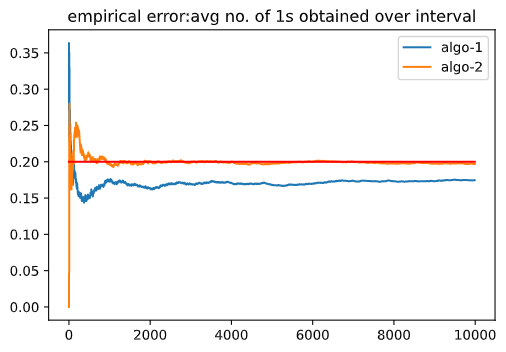
\includegraphics[scale=0.4]{68-comb-err.png}
     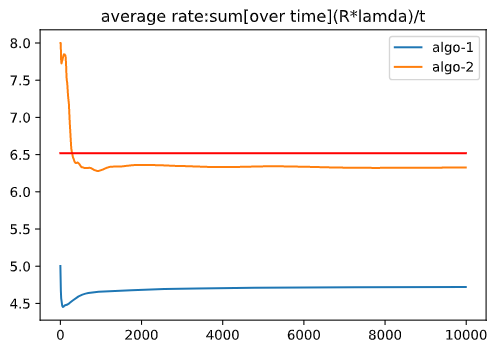
\includegraphics[scale=0.4]{68-comb-rate.png}
     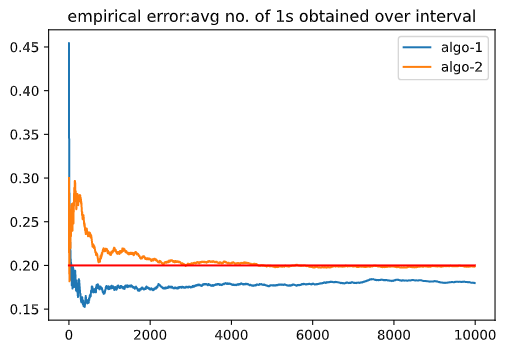
\includegraphics[scale=0.4]{1012-comb-err.png}
     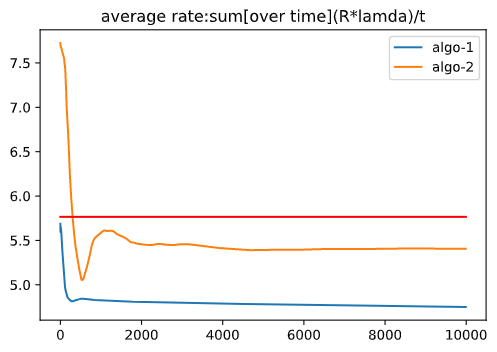
\includegraphics[scale=0.4]{1012-comb-rate.png}
     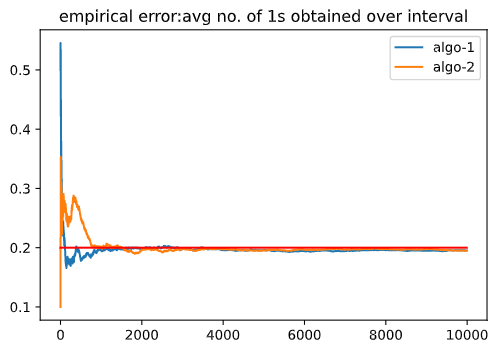
\includegraphics[scale=0.4]{1520-comb-err.png}
     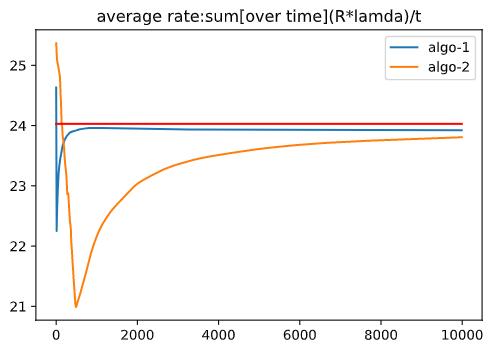
\includegraphics[scale=0.4]{1520-comb-rate.png}
     \caption {Plots of empirical error(left) and average reward(right) of sample test-beds with (en,ch, tol) values equal to (6,8,.2), (10,12,.25), (15,20,.2) respectively when algorithms 1 and 2 are used}
   \label{fig:comb}
   \end{center}
\end{figure} 

\begin{figure}[H]
    \begin{center}
      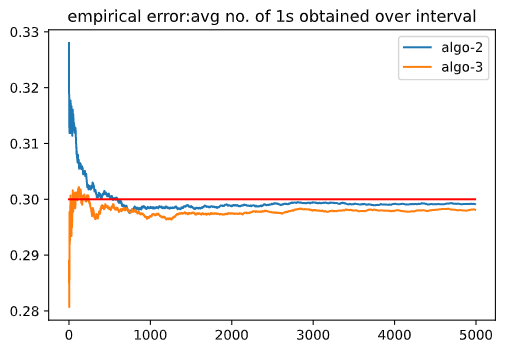
\includegraphics[scale=0.4]{33-m-err.png}
      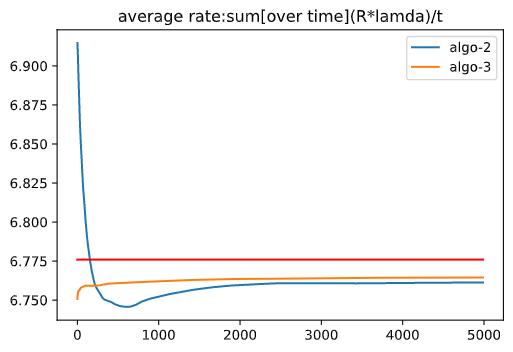
\includegraphics[scale=0.4]{33-m-rate.png}
      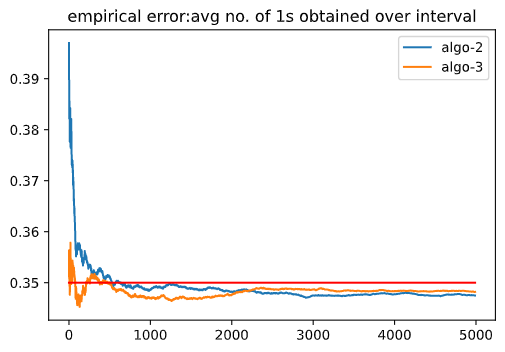
\includegraphics[scale=0.4]{45-m-err.png}
      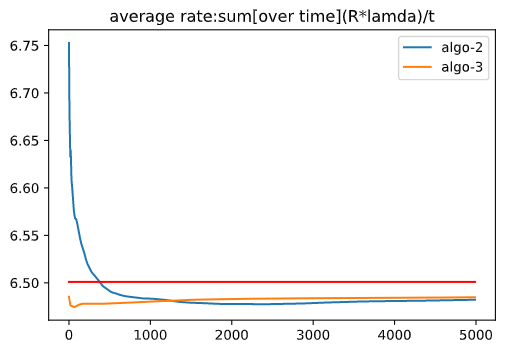
\includegraphics[scale=0.4]{45-m-rate.png}
      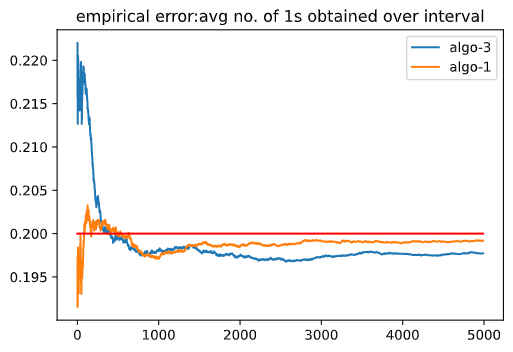
\includegraphics[scale=0.4]{68-m-err.png}
      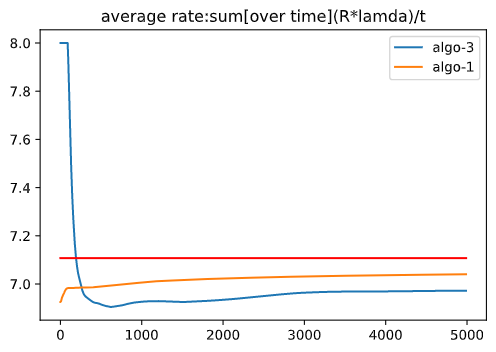
\includegraphics[scale=0.4]{68-m-rate.png}
      \caption {Plots of empirical error(left) and average reward(right) of sample test-beds with Markov channel probabilities and (en,ch,tol) values equal to (3,3,.3), (4,5,.35), (6,8,.2) respectively when algorithm 3 is used}
    \label{fig:m}
    \end{center}
 \end{figure}

\section{Conclusion and Future Work}
We see that algorithms 1 and 2 can be deployed based on the use case like whether we want a safe/reliable system or the one with better rates. These algorithms were producing decent results but theoretically we weren't able to prove their convergence. We showed that there is bound on regret at each round in Regret Analysis section but that doesn't address the convergence seen. We can see from \ref{fig:comb} that within reasonable number of rounds the gap between $r_t$ and $r_*$ is decresing. We might include case:1 probability to get better bound. Let this probability be $1-\epsilon$, then the regret bound we obtained will be of the form $\epsilon$ times regret in the case:2. If we were able to show that this $\epsilon$ a decreasing function of time then that can be used to bound regret. This is the direction we see the future work going. 

%%%%%%%%%%%%%%%%%%%%%%%%%%%%%%%%%%%%%%%%%%%%%%%%%%%%%%%%%%%%
% Appendices.

 \appendix
 
 \chapter{I}
 
 INTRODUCTION - Page 1 \\
 Problem Formulation - Page 2 \\
 Algorithm - Page 2 \\
 Regret Analysis - Page 4 \\
 Some More Algorithms - Page 7 \\
 Results - Page 8 \\
 Conclusion and Future Work - Page 11 \\
 

%%%%%%%%%%%%%%%%%%%%%%%%%%%%%%%%%%%%%%%%%%%%%%%%%%%%%%%%%%%%
% List of papers

%%%%%%%%%%%%%%%%%%%%%%%%%%%%%%%%%%%%%%%%%%%%%%%%%%%%%%%%%%%%
% List of papers

\listofpapers

\begin{enumerate}  
	\item Aldo Pacchiano and Mohammad Ghavamzadeh and Peter Bartlett and Heinrich Jiang, \newblock
	Stochastic Bandits with Linear Constraints,
	\newblock {\em Proceedings of The 24th International Conference on Artificial Intelligence and Statistics, PMLR 130:2827-2835}, (2020).
    \item Yasin Abbasi-yadkori and Dávid Pál and Csaba Szepesvári, \newblock
    Improved Algorithms for Linear Stochastic Bandits,
    \newblock {\em Advances in Neural Information Processing Systems 24 (NIPS)}, (2011).
\end{enumerate}  

%%%%%%%%%%%%%%%%%%%%%%%%%%%%%%%%%%%%%%%%%%%%%%%%%%%%%%%%%%%%
% Bibliography.
\pagebreak
\begin{singlespace}
  \begin{small}
	\bibliography{refs}
  \end{small}
\end{singlespace}


\end{document}



